\chapter{Design}
	\section{Overall system design}
\begin{center}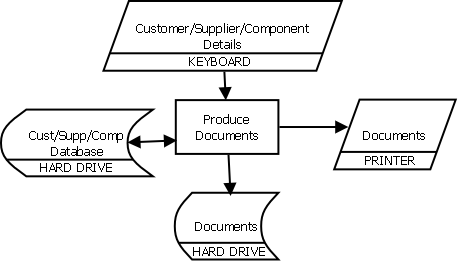
\includegraphics[scale=0.5]{systemsflowchart}\end{center}
	\section{Description of modular system structure}
\begin{center}
	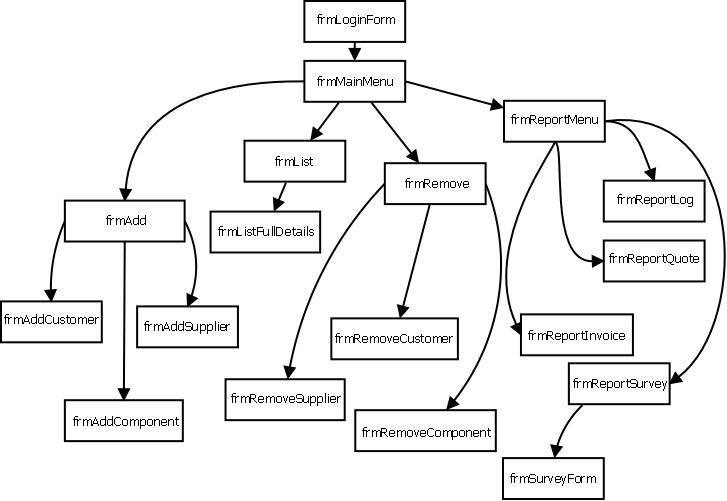
\includegraphics[scale=0.5]{hcfinal}
\end{center}
	\begin{center}
		\begin{tabular}{| p{4cm} | p{4cm} | p{4cm} | p{4cm} | }
			\hline
			\textbf{Input} & \textbf{Process} & \textbf{Storage} & \textbf{Output}\\
			\hline
			Customer data & Validation & Customer table in the database & \\
			\hline
			Supplier data & Validation & Supplier table in the database & \\
			\hline
			Component data & Validation & Component table in the database & \\
			\hline
			Survey details & Validation & Installation table in the database & \\
			\hline
			Selected customer & Microsoft Word opens, the program having executed code to make the quotation or invoice & A Microsoft Word document & A Microsoft Word document containing customer details\\
			\hline
			Selected log form & Microsoft Word opens, the program having executed code to open the selected log form & A Microsoft Word document & A Microsoft Word document containing the various log tables\\
			\hline
		\end{tabular}
	\end{center}
	\section{Design data dictionary}
Customer:
\begin{center}
	\begin{longtable}{ | p{3cm} | p{3cm} | p{2cm} | p{1cm} | p{2cm} | p{2cm} | p{2cm} | }
		\hline
		\textbf{Field Name} & \textbf{Example} & \textbf{Data Type}
& \textbf{Size (chars.)} & \textbf{Validation} & \textbf{Default Value} & \textbf{Key Field}\\
		\endfirsthead
		\hline
		\textbf{Field Name (cont.)} & \textbf{Example (cont.)} &
\textbf{Data Type (cont.)} & \textbf{Size (chars.) (cont.)} & \textbf{Validation (cont.)} & \textbf{Default Value (cont.)} & \textbf{Key Field (cont.)}\\
		\endhead
		\hline
		cust\_id & 1 & Autonumber & 4 & Filled automatically & Increment by 1 as customers are added & Primary key\\
		\hline
		cust\_title & Mr & String & 4 & $\neq$ NULL & &\\
		\hline
		cust\_name & Joe Bloggs & String & 50 & $\neq$ NULL & &\\
		\hline
		cust\_billaddress & 25 BillingAddress Place & String & 50 & $\neq$ NULL & &\\
		\hline
		cust\_billpostcode & JE49 8RH & String & 8 & $\neq$ NULL & &\\
		\hline
		cust\_instaddress & 26 InstallAddress Place & String & 50 & $\neq$ NULL if $\neq$ BillAddress & &\\
		\hline
		cust\_instpostcode & IP38 9FJ & String & 8 & $\neq$ NULL if $\neq$ BillPostcode & &\\
		\hline
		cust\_hometelno & 01234 567890 & String & 12 & $\neq$ NULL & &\\
		\hline
		cust\_mobtelno & 07890 098765 & String & 12 & $\neq$ NULL & &\\
		\hline
		cust\_email & x@y.com & String & 25 & Must contain `@' & &\\
		\hline
		cust\_mpan & 12345789012334 & String & 14 & Erroneous if length $\neq$ 14 & &\\
		\hline
	\end{longtable}
\end{center}

Supplier:
\begin{center}
	\begin{longtable}{ | p{3cm} | p{3cm} | p{2cm} | p{1cm} | p{2cm} | p{2cm} | p{2cm} | }
		\hline
		\textbf{Field Name} & \textbf{Example} & \textbf{Data Type}
& \textbf{Size (chars.)} & \textbf{Validation} & \textbf{Default Value} & \textbf{Key Field}\\
		\endfirsthead
		\hline
		\textbf{Field Name (cont.)} & \textbf{Example (cont.)} &
\textbf{Data Type (cont.)} & \textbf{Size (chars.) (cont.)} & \textbf{Validation (cont.)} & \textbf{Default Value (cont.)} & \textbf{Key Field (cont.)}\\
		\endhead
		\hline
		supp\_id & 1 & Autonumber & 4 & Filled automatically by the database & Increment by 1 as suppliers are added & Primary key\\
		\hline
		supp\_name & Alternergy & String & 25 & $\neq$ NULL & &\\
		\hline
		supp\_address & 25 Supplier Place & String & 50 & $\neq$ NULL & &\\
		\hline
		supp\_postcode & N1 8YE & String & 15 & $\neq$ NULL & &\\
		\hline
		sup\_telno & 03739 974636 & String & 13 & $\neq$ NULL & &\\
		\hline
		supp\_contactname & Joe Bloggs & String & 25 & Can $=$ 0 & &\\
		\hline
	\end{longtable}
\end{center}

Component:
\begin{center}
	\begin{longtable}{ | p{3cm} | p{3cm} | p{2cm} | p{1cm} | p{2cm} | p{2cm} | p{2cm} | }
		\hline
		\textbf{Field Name} & \textbf{Example} & \textbf{Data Type}
& \textbf{Size (chars.)} & \textbf{Validation} & \textbf{Default Value} & \textbf{Key Field}\\
		\endfirsthead
		\hline
		\textbf{Field Name (cont.)} & \textbf{Example (cont.)} &
\textbf{Data Type (cont.)} & \textbf{Size (chars.) (cont.)} & \textbf{Validation (cont.)} & \textbf{Default Value (cont.)} & \textbf{Key Field (cont.)}\\
		\endhead
		\hline
		comp\_id & 1 & Autonumber & 4 & Filled automatically in the database & Increment by 1 as components are added & Primary key\\
		\hline
		comp\_name & Suntech 250 & String & 50 & $\neq$ NULL & &\\
		\hline
		comp\_type & Solar Panel & String & 50 & $\neq$ NULL & &\\
		\hline
		comp\_serialno & SEN1023854 & String & 10 & $\neq$ NULL & &\\
		\hline
		comp\_panelwp & 3.25 & Integer & 32 (bits) & $\neq$ NULL, type check: integer & &\\
		\hline
		comp\_supplier & & & & & Foreign key, filled from supplier table & Foreign key\\
		\hline
	\end{longtable}
\end{center}

Installation:

\begin{center}
	\begin{longtable}{ | p{3cm} | p{3cm} | p{2cm} | p{1cm} | p{2cm} | p{2cm} | p{2cm} | }
		\hline
		\textbf{Field Name} & \textbf{Example} & \textbf{Data Type} & \textbf{Size} & \textbf{Validation} & \textbf{Default Value} & \textbf{Key Field}\\
		\endfirsthead
		\hline
		\textbf{Field Name (cont.)} & \textbf{Example (cont.)} & \textbf{Data Type (cont.)} & \textbf{Size (cont.)} & \textbf{Validation (cont.)} & \textbf{Default Value (cont.)} & \textbf{Key Field (cont.)}\\
		\endhead
		\hline
		inst\_id & 1 & Autonumber & 4 & Filled automatically & Increment by 1 as installation details are added & Primary Key\\
		\hline
		inst\_quoteno & 5 & Integer & 32 (bits) & Filled automatically & Increment by 1 every time a quote is created &\\
		\hline
		inst\_netprice & 8 000 & Integer & 32 (bits) & $\neq$ NULL, type check: integer & &\\
		\hline
		inst\_vat & 5.00\% & Integer & 32 (bits) & & 5.00\%, type check: integer &\\
		\hline
		inst\_totalprice & 15 000 & Integer & 32 (bits) & $\neq$ NULL, type check: integer & &\\
		\hline
		inst\_deposit & 1 000 & Integer & 32 (bits) & $\neq$ NULL, type check: integer & &\\
		\hline
		inst\_dateinstall & 04\slash 01\slash 12 & Date & 10 & Can be NULL if customer doesn't agree to install & &\\
		\hline
		inst\_sapcalc & 0.8$\times$2.9$\times$1073$\times$0.8 & Integer & 32 (bits) & $\neq$ NULL & &\\
		\hline
		inst\_purchordernum & 1230201 & Integer & 32 (bits) & $\neq$ NULL, type check: integer & &\\
		\hline
		inst\_deliverydate & 03\slash 01\slash 12 & Date & 10 & $\neq$ NULL & &\\
		\hline
		inst\_invoiceno & 1 & Integer & 32 (bits) & Filled automatically & Increment by 1 every time an invoice is created &\\
		\hline
		cust\_id & & & & & Foreign key, filled from customer table & Foreign key\\
		\hline
	\end{longtable}
\end{center}

	\section{Database design}
\begin{center}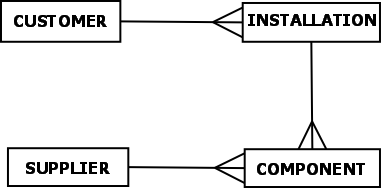
\includegraphics[scale=0.45]{erd_new}\end{center}
	
Every customer can have many installations; Each installation can only be
installed on one customer's roof.\\
Every installation can have many components. Each component can only be
fitted onto one installation.\\
Every supplier can supply many components.  Each component can only be
supplied by one, specialist supplier (the best one).

	\textit{Customer}(\underline{cust\_id}, cust\_title, cust\_name, cust\_billaddress, cust\_billpostcode, cust\_instaddress, cust\_instpostcode, cust\_hometelno, cust\_mobtelno, cust\_mpan, cust\_email)\\
	\textit{Supplier}(\underline{supp\_id}, supp\_name, supp\_address, supp\_postcode, supp\_telno, supp\_contactname)\\
	\textit{Component}(\underline{comp\_id}, comp\_name, comp\_type, comp\_serialno, comp\_panelwp, comp\_supplier*)\\
	\textit{Installation}(\underline{inst\_id}, inst\_netprice, inst\_vat, inst\_totalprice, inst\_deposit, inst\_dateinstall, inst\_sapcalc, inst\_purchordernum, inst\_deliverydate, inst\_invoiceno, cust\_id*)

	This database is in the first normal form (1NF) because every piece of data is atomic, i.e. there are no repeating groups.\\
	The database is in the second normal form (2NF) because it is in the first normal form (1NF) and there are no partial key dependencies.\\
	The database is in the third normal form (3NF) because it is in the second normal form (2NF) and contains no non-key dependencies.
	\section{File organisation and processing}
The system requires a Microsoft Access database to work, and various
reports to produce the invoices, quotes and log sheets in Microsoft Word document files.  These reports, however, cannot be deleted unless
they can be easily reproduced with the same data, but the size of each
report is going to be more or less the same---just documents with content but no headed paper as it will get printed onto headed paper.

The maximum file storage requirement per year for the database would be 10 000 KB. (Formula: The average row will take up 20KB of space, and SFS estimate 500 records per year, so a maximum of 10 000 KB per year.)\\ 
The maximum file storage requirement per year for the reports would be 25 000 KB. (Formula: The average quotation is 25 KB in size, with both a quotation and an invoice for each of the 500 customers, so a maximum of 25 000 KB per year.)
	\section{Identification of storage media}
Stored on one computer's hard drive, and the database files will be backed
up regularly to an external hard drive as well as daily and automatically
to Dropbox, when changed.  I am choosing a hard drive as a storage medium as the files are quite small and the desktop hard drive that SFS have is big enough.  The database only has to be stored on one computer as the program is only going to be used from one computer, and the documents produced can be easily emailed or put into Dropbox sharing if they need to be shared between Philip or Angi or any other eventual employees.

	\section{Identification of suitable algorithms for data transformation, and pseudocode of those algorithms}
Validation:
\begin{algorithmic}
        \If {$NameTextBox \gets ""$}
                $MsgBox("Enter\ a\ name!")$
        \EndIf
\end{algorithmic}

Opening a Microsoft Word document:
\begin{algorithmic}
        \If {$dateselection \gets "December\ 2011"$}
                \State $docopened \gets Open("log\_dec11.docx")$
        \EndIf
\end{algorithmic}

Bubble sort for the customers, also implementable for suppliers and components by changing `cust\_name' to `supp\_name' and `comp\_name' respectively:
\begin{algorithmic}
	\Repeat
		\State $swapped \gets false$
		\For {$i \gets 0 \to length(cust\_name) - 1$}
			\If {$cust\_name[i - 1] > cust\_name[i]$}
				\State $swap(cust\_name[i - 1], cust\_name[i])$
				\State $swapped \gets true$
			\EndIf
		\EndFor
	\Until $swapped \gets false$ 
\end{algorithmic}

\textbf{Some SQL:}

Selecting all customers:
\begin{verbatim} 
        SELECT * FROM Customer
\end{verbatim}
Search for a customer:
\begin{verbatim}
	SELECT cust_name FROM Customer WHERE cust_name LIKE '%" & search_text "%''
\end{verbatim}
Insert customer details:
\begin{verbatim}
        INSERT INTO Customer (cust_title, cust_name, cust_billaddress,
        cust_billpostcode, cust_instaddress, cust_instpostcode,
        cust_hometelno, cust_mobtelno, cust_mpan, cust_email) &
        VALUES (@cust_title,@cust_name,@cust_billaddress,
        @cust_billpostcode,@cust_instaddress,@cust_instpostcode,
        @cust_hometelno,@cust_mobtelno,@cust_mpan,@cust_email)
\end{verbatim}
Delete a supplier:
\begin{verbatim}
	DELETE * FROM Supplier WHERE supp\_name = " & selectedname & ""
\end{verbatim}
	\section{Class definitions}
Not applicable.
	\section{User interface rationale}
\begin{itemize}
	\item{Graphical user interface:}
	\begin{itemize}
		\item{Buttons.}
		\item{Drop down menus for finite choices that the user can select, so that the user does not have to remmeber the right names for things like `Customer' vs. `Customers' in some places, to enable easy selection.}
		\item{Textboxes lined up with labels, for easy data entry.}
	\end{itemize}
	\item{Font:}
	\begin{itemize}
		\item{Forms: sans-serif, size 8.5.  Sans-serif fonts are easier on the eye and look professional.}
		\item{Report documents: Calibri, size 22 for the headers, size 11 for the main text.  Sans-serif fonts are easier on the eye and look professional.}
	\end{itemize}
	\item{Colours: grey, black, blue.  I am using these colours as they keep the program clear, simple and easy to read and use.}
\end{itemize}
	\section{User interface sample of planned data capture and data entry designs}
The main menu:

\begin{center}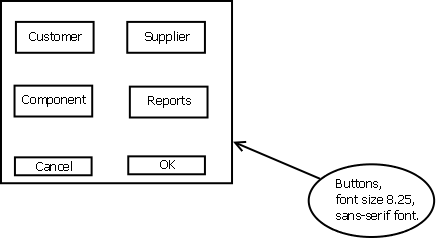
\includegraphics[scale=0.5]{mainmenudesignoriginal.png}\end{center}
	
The customer entry form:

\begin{center}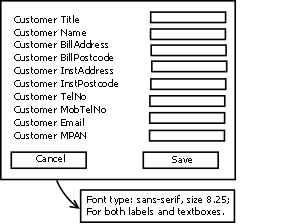
\includegraphics{custentrydesignoriginal.png}\end{center}
	\section{User interface sample of planned output designs}
Invoice:

\begin{center}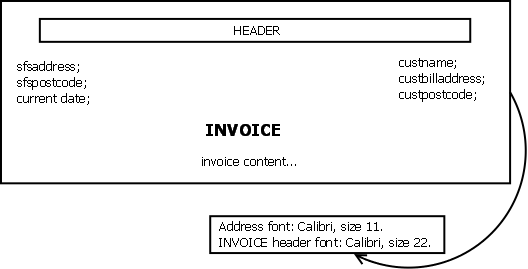
\includegraphics[scale=0.5]{invoicedesignoriginal.png}\end{center}

Log form:

\begin{center}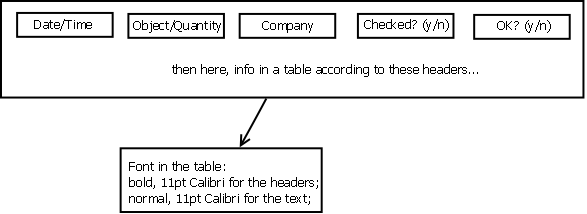
\includegraphics[scale=0.5]{logdesignoriginal.png}\end{center}
	\section{Description of measures planned for security and integrity of data}
If the user's computer crashed, they would be able to restore program files from a recent backup.  These backups would be taken daily in accordance with SFS's file backup procedure, onto an external harddrive, and to Dropbox.  Every user will have access to all parts of the system as all parts are important to each of the (two) users.  The program itself will be password protected with a login screen, and the database containing the login details stored in a location not immediately obvious---the user will not need to look at the database unless he or she forgets his or her password.  The files---invoices, quotations and log forms can be edited by any user of the computer who has write access to the directory they are stored in---usually only Angi would edit them though.
	\section{Descriptions of measures planned for systems security}
One computer will contain the database and only one person will be using the system at any one time, because only one person will be in front of the computer that it will be installed on typing.  If the system was to be used on multiple computers, multiple copies of the database would exist and no-one would know which was the current version, so they would get very confused.  In terms of systems security, the computer and the program itself will be password protected.  If the computer dies completely or burns down, Dropbox will receive copies of the data files so they can be restored on the new computer that will have to be bought, and the program will have to be reinstalled.
	\section{Overall test strategy}
	
First I will test the flow of control, i.e. that the forms all link to one another and every button works.  This is top down testing.\\
Next, I will test the input validation, i.e. whether the user input validates and blank textboxes or erroneous data produce error messages, on all of the forms.  This is white box testing.\\
Then, I will again test the flow of control with reference to the tab order of the textboxes.  This is again top down testing.\\
I will also test any searching that I implement, with some black box testing, and also some testing that none of the database code crashes.\\
My final test will be that the Word documents open with the correct data and formatting required by the user, and are able to be edited, saved, and printed.